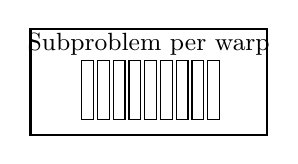
\begin{tikzpicture}[every node/.style={thick,rectangle,inner sep=0pt}]

\def \dx {0.05}
\def \dy {0.2}
\def \recx {0.15}
\def \recX {9*\recx + 10*\dx}
\def \recy {0.75}
\def \recY {\recy + 3 * \dy}

%% left child 
\draw [black] (0 + 0, 0 + 0) rectangle (0 + \recx, 0 + \recy);
\draw [black] (0 + \recx + \dx, 0) rectangle (0 + 2*\recx + \dx, 0 + \recy);
\draw [black] (0 + 2*\recx + 2*\dx, 0 + 0) rectangle (0 + 3*\recx + 2*\dx, 0 + \recy);
\draw [black] (0 + 3*\recx + 3*\dx, 0 + 0) rectangle (4*\recx + 3*\dx, 0 + \recy);
\draw [black] (0 + 4*\recx + 4*\dx, 0 + 0) rectangle (5*\recx + 4*\dx, 0 + \recy);
\draw [black] (0 + 5*\recx + 5*\dx, 0 + 0) rectangle (6*\recx + 5*\dx, 0 + \recy);
\draw [black] (0 + 6*\recx + 6*\dx, 0 + 0) rectangle (7*\recx + 6*\dx, 0 + \recy);
\draw [black] (0 + 7*\recx + 7*\dx, 0 + 0) rectangle (8*\recx + 7*\dx, 0 + \recy);
\draw [black] (0 + 8*\recx + 8*\dx, 0 + 0) rectangle (9*\recx + 8*\dx, 0 + \recy);

\draw[thick, black] (0-13*\dx, 0-\dy) rectangle (0-13*\dx + \recX + 23 * \dx, 0-\dy + \recY);
\node () at (0 + 5 * \recx + 2 * \dx, \recy + \dy) {\small Subproblem per warp};

\end{tikzpicture}